\documentclass[12pt]{beamer}
\usepackage{Estilos/BeamerFC}
\usepackage{Estilos/ColoresLatex}
\usetheme{Warsaw}
\usecolortheme{seahorse}
%\useoutertheme{default}
\setbeamercovered{invisible}
% or whatever (possibly just delete it)
\setbeamertemplate{section in toc}[sections numbered]
\setbeamertemplate{subsection in toc}[subsections numbered]
\setbeamertemplate{subsection in toc}{\leavevmode\leftskip=3.2em\rlap{\hskip-2em\inserttocsectionnumber.\inserttocsubsectionnumber}\inserttocsubsection\par}
\setbeamercolor{section in toc}{fg=blue}
\setbeamercolor{subsection in toc}{fg=blue}
\setbeamercolor{frametitle}{fg=blue}
\setbeamertemplate{caption}[numbered]

\setbeamertemplate{footline}
\beamertemplatenavigationsymbolsempty
\setbeamertemplate{headline}{}


\makeatletter
\setbeamercolor{section in foot}{bg=gray!30, fg=black!90!orange}
\setbeamercolor{subsection in foot}{bg=blue!30}
\setbeamercolor{date in foot}{bg=black}
\setbeamertemplate{footline}
{
  \leavevmode%
  \hbox{%
  \begin{beamercolorbox}[wd=.333333\paperwidth,ht=2.25ex,dp=1ex,center]{section in foot}%
    \usebeamerfont{section in foot} \insertsection
  \end{beamercolorbox}%
  \begin{beamercolorbox}[wd=.333333\paperwidth,ht=2.25ex,dp=1ex,center]{subsection in foot}%
    \usebeamerfont{subsection in foot}  \insertsubsection
  \end{beamercolorbox}%
  \begin{beamercolorbox}[wd=.333333\paperwidth,ht=2.25ex,dp=1ex,right]{date in head/foot}%
    \usebeamerfont{date in head/foot} {T1 - Segunda presentación} \hspace*{2em}
    \insertframenumber{} / \inserttotalframenumber \hspace*{2ex} 
  \end{beamercolorbox}}%
  \vskip0pt%
}
\makeatother

\makeatletter
\patchcmd{\beamer@sectionintoc}{\vskip1.5em}{\vskip0.8em}{}{}
\makeatother
\usepackage{pifont}
\newcommand{\cmark}{\ding{51}}%
\newcommand{\xmark}{\ding{55}}%

\makeatletter
\setbeamertemplate{footline}
{
  \leavevmode%
  \hbox{%
  \begin{beamercolorbox}[wd=.333333\paperwidth,ht=2.25ex,dp=1ex,center]{section in foot}%
    \usebeamerfont{section in foot} \insertsection
  \end{beamercolorbox}%
  \begin{beamercolorbox}[wd=.333333\paperwidth,ht=2.25ex,dp=1ex,center]{subsection in foot}%
    \usebeamerfont{subsection in foot}  \insertsubsection
  \end{beamercolorbox}%
  \begin{beamercolorbox}[wd=.333333\paperwidth,ht=2.25ex,dp=1ex,right]{date in head/foot}%
    \usebeamerfont{date in head/foot} \insertshortdate{} \hspace*{2em}
    \insertframenumber{} / \inserttotalframenumber \hspace*{2ex} 
  \end{beamercolorbox}}%
  \vskip0pt%
}
\makeatother

\sisetup{
  per-mode=fraction,
  fraction-function=\tfrac
}

\setbeamertemplate{navigation symbols}{}
\date{27 de abril}

% \sisetup{math-rm=\symup,detect-all}
\sisetup{detect-all, math-rm = \ensuremath}

\title{Sesión 10. Física}
\subtitle{Asesoría}

\begin{document}

\maketitle
\fontsize{14}{14}\selectfont
\spanishdecimal{.}

\section*{Contenido}
\frame[allowframebreaks]{\tableofcontents[currentsection, hideallsubsections]}

\section{Primera condición de equilibrio}
\frame{\tableofcontents[currentsection, hideothersubsections]}
\subsection{Ejercio 8 - Guía}

\begin{frame}
\frametitle{Enunciado del Ejercicio 8}
Un anuncio de \SI{200}{\newton} se cuelga de un techo como se muestra en la figura, de manera que las cuerdas que lo sostienen forman un ángulo de \ang{90}.
\\
\bigskip
\pause
¿Cuál es la tensión en cada segmnento de la cuerda?
\end{frame}
\begin{frame}
\frametitle{Figura del Ejercicio 8}
\begin{figure}
  \centering
  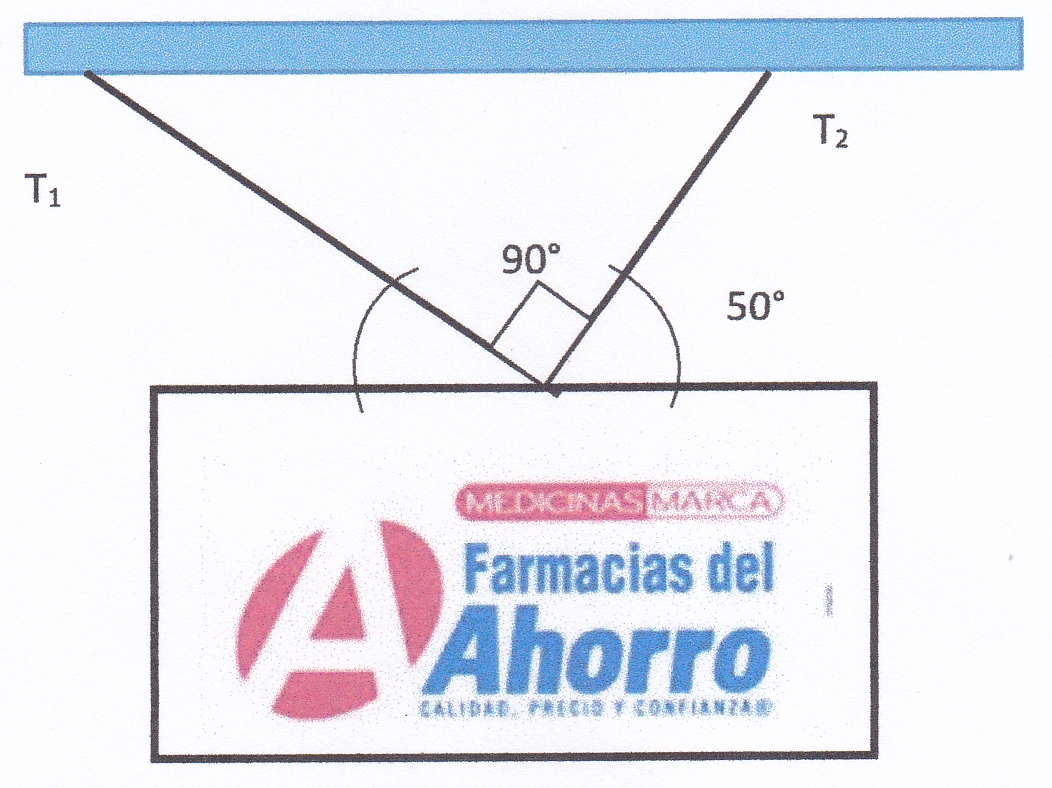
\includegraphics[scale=0.9]{Imagenes/DCL_Problema_08.png}
\end{figure}
\end{frame}
\begin{frame}
\frametitle{Construyedo el DCL}
Para el DCL debemos de considerar las fuerzas involucradas en el ejercicio, tomemos en cuenta que: \pause el enunciado nos indica el peso del anuncio:
\begin{align*}
W = \SI{200}{\newton}
\end{align*}
\end{frame}
\begin{frame}
\frametitle{Construyedo el DCL}
Así mismo, sabemos cuánto vale el ángulo que se forma entre la cuerda $1$ y la parte superior del anuncio:
\pause
\begin{eqnarray*}
\begin{aligned}
\theta_{1} &+ \ang{90} + \theta_{2} = \ang{180} \\[0.5em] \pause
\theta_{1} &= \ang{180} - \ang{90} - \theta_{2} = \\[0.5em] \pause
\theta_{1} &= \ang{180} - \ang{90} - \ang{50} = \\[0.5em] \pause
\theta_{1} &= \ang{40}
\end{aligned}
\end{eqnarray*} 
\end{frame}
\begin{frame}
\frametitle{Diagrama de cuerpo libre}
\begin{figure}
\centering
\begin{tikzpicture}[scale=1.3]
  \draw (-1, 0) -- (1.5, 0);
  \draw [-stealth, thick, color=ao](0, 0) -- (0, -2) node [right, midway] {\small{$-W$}};
  
  \pause
  \draw [thick, -stealth, color=red] (0, 0) -- (0.986, 1.175) node [above=0.1, midway] {\small{$T_{2}$}};
  \draw (-1.4, 1.175) -- (1.2, 1.175);
  % \draw (0.986, 1.175) -- (-0.985, 0.5);
  \draw [color=red] (0.5, 0) arc(0:50:0.5);
  \node at (0.7, 0.2) [color=red] {\small{$\theta_{2}$}};

  \pause
  \draw [thick, -stealth, color=red] (0, 0) -- (-0.985, 1.175) node [above, midway] {\small{$T_{1}$}};
  
  \draw [color=red] (-0.4, 0) arc(180:130:0.4);
  \node at (-0.6, 0.2) [color=red] {\small{$\theta_{1}$}};

\end{tikzpicture}
\end{figure}
\end{frame}
\begin{frame}
\frametitle{Listando las fuerzas}
Presentamos la tabla con las fuerzas involucradas y los ángulos que forman:
\pause
\begin{table}
\centering
\begin{tabular}{c | c}
Fuerza & Ángulo \\ \hline
$T_{1}$ & \ang{40} \\ \hline
$T_{2}$ & \ang{50} \\ \hline
$W$ & \ang{270} \\ \hline
\end{tabular}
\end{table}
\end{frame}
\begin{frame}
\frametitle{Descomponiendo los vectores}
Ahora procedemos a hacer la descomposición de los vectores tanto en la dirección del eje $x$ como del eje $y$.
\end{frame}
\begin{frame}
\frametitle{Descomponiendo los vectores}
\begin{table}
\centering
\begin{tabular}{c | c | c}
Componente & Expresión & Sustitución \\ \hline
$T_{1x}$ & $(- \cos \ang{40})(T_{1})$ & $(-0.766) (T_{1})$ \\ \hline
$T_{1y}$ & $(\sin \ang{40})(T_{1})$ & $(0.642) (T_{1})$ \\ \hline
$T_{2x}$ & $(\cos \ang{50})(T_{2})$ & $(0.642) (T_{2})$ \\ \hline
$T_{2y}$ & $(\sin \ang{50})(T_{2})$ & $(0.766) (T_{2})$ \\ \hline
\end{tabular}
\end{table}
\end{frame}
\begin{frame}
\frametitle{Descomponiendo los vectores}
\begin{table}
\centering
\begin{tabular}{c | c | c}
Componente & Expresión & Sustitución \\ \hline
$W_{x}$ & $(\cos \ang{270})(W)$ & $(0) (W)$ \\ \hline
$W_{y}$ & $(\sin \ang{270})(W)$ & $(-1) (\SI{200}{\newton})$ \\ \hline
\end{tabular}
\end{table}
\end{frame}
\begin{frame}
\frametitle{Condición de equilibrio}
Ya hemos revisado que la primera condición de equilibrio se presenta cuando:
\pause
\begin{align*}
\nsum F_{x} &= 0 \\
\nsum F_{y} &= 0
\end{align*}
\end{frame}
\begin{frame}
\frametitle{Suma de las componentes en $x$}
Para la componente en $x$:
\pause
\begin{eqnarray*}
\begin{aligned}
\nsum F_{x} &= 0 \\ \pause
&= T_{1x} + T_{2x} + W_{x} = 0 \\ \pause
&(-0.766)(T_{1}) + (0.642)(T_{2}) + 0 = 0 \\  \pause
&(-0.766)(T_{1}) + (0.642)(T_{2}) = 0
\end{aligned}
\end{eqnarray*}
\end{frame}
\begin{frame}
\frametitle{Suma de las componentes en $y$}
Para la componente en $y$:
\pause
\begin{eqnarray*}
\begin{aligned}
\nsum F_{y} &= 0 \\ \pause
&= T_{1y} + T_{2y} + W_{y} = 0 \\ \pause
&(0.642)(T_{1}) + (0.766)(T_{2}) - \SI{200}{\newton} = 0
\end{aligned}
\end{eqnarray*}
\end{frame}
\begin{frame}
\frametitle{Sistema de ecuaciones}
Hemos obtenido el siguiente sistema simultáneo de ecuaciones:
\pause
\begin{align}
(-0.766)(T_{1}) + (0.642)(T_{2}) &= 0 \label{eq:ecuacion_08_01} \\[0.5em]
(0.642)(T_{1}) + (0.766)(T_{2}) - \SI{200}{\newton} &= 0 \label{eq:ecuacion_08_02}
\end{align}
\end{frame}
\begin{frame}
\frametitle{Resolviendo el sistema de ecuaciones}
De la ec. (\ref{eq:ecuacion_08_01}) despejamos $T_{2}$:
\pause
\begin{eqnarray*}
\begin{aligned}
(-0.766)(T_{1}) + (0.642)(T_{2}) &= 0 \\[0.5em] \pause
(0.642)(T_{2}) &= (0.766)(T_{1}) = \\[0.5em] \pause
T_{2} &= \dfrac{0.766}{(0.642)} \cdot T_{1} = \\[0.5em] \pause
T_{2} &= 1.193 \cdot T_{1}
\end{aligned}
\end{eqnarray*}
\end{frame}
\begin{frame}
\frametitle{Sustituyendo el valor}
Ahora ya podemos obtener el valor de la tensión $T_{1}$ usando la ec. (\ref{eq:ecuacion_08_02}):
\pause
\begin{eqnarray*}
\begin{aligned}
(0.642)(T_{1}) + (0.766)(T_{2}) - \SI{200}{\newton} &= 0 \\[0.5em] \pause
(0.642)(T_{1}) + (0.766)(1.193 \cdot T_{1}) - \SI{200}{\newton} &= 0 \\[0.5em] \pause
(0.642)(T_{1}) + (0.913)(T_{1}) - \SI{200}{\newton} &= 0 \\[0.5em] \pause
(1.555)(T_{1}) - \SI{200}{\newton} &= 0 \\[0.5em] \pause
(1.555)(T_{1}) &= \SI{200}{\newton}
\end{aligned}
\end{eqnarray*}
\end{frame}
\begin{frame}
\frametitle{Sustituyendo el valor}
\begin{eqnarray*}
\begin{aligned}
T_{1} &= \dfrac{\SI{200}{\newton}}{1.555} = \\[0.5em] \pause
T_{1} &= \SI{128.61}{\newton}
\end{aligned}
\end{eqnarray*}
\end{frame}
\begin{frame}
\frametitle{Recuperando el segundo valor}
Ahora podemos ocupar el valor de $T_{1}$ para obtener el valor de la tensión $T_{2}$, con la ec. (\ref{eq:ecuacion_08_01}):
\pause
\begin{eqnarray*}
\begin{aligned}
(-0.766)(T_{1}) + (0.642)(T_{2}) &= 0 \\[0.5em] \pause
(-0.766)(\SI{128.61}{\newton}) + (0.642)(T_{2}) &= 0 \\[0.5em] \pause
- \SI{98.51}{\newton} + (0.642)(T_{2}) &= 0 \\[0.5em] \pause
(0.642)(T_{2}) &= \SI{98.51}{\newton}
\end{aligned}
\end{eqnarray*}
\end{frame}
\begin{frame}
\frametitle{Recuperando el segundo valor}
\begin{eqnarray*}
\begin{aligned}
T_{2} &= \dfrac{\SI{98.51}{\newton}}{0.642} \\[0.5em] \pause
T_{2} &= \SI{153.44}{\newton}
\end{aligned}
\end{eqnarray*}
\end{frame}
\begin{frame}
\frametitle{Solución completa}
Hemos obtenido las tensiones en las cuerdas que soportan el anuncio:
\begin{align*}
T_{1} &= \SI{128.61}{\newton} \\[0.5em]
T_{2} &= \SI{153.44}{\newton}
\end{align*}
\end{frame}

\section{Segunda condición de equilibrio}
\frame{\tableofcontents[currentsection, hideothersubsections]}
\subsection{Definición}

\begin{frame}
\frametitle{Definición}
La \textocolor{blue}{segunda condición de equilibrio}, \pause también conocido como \textocolor{red}{condición de equilibrio rotacional}, \pause es una condición en la que un objeto o sistema en rotación se mantiene en reposo o en un movimiento de rotación constante y uniforme.
\end{frame}
% \begin{frame}
% \frametitle{Segunda condición}
% En otras palabras, \pause el objeto o sistema no experimenta una aceleración angular neta, \pause lo que significa que \textocolor{carmine}{la suma de todas las fuerzas y momentos} que actúan sobre el objeto o sistema \pause \textocolor{byzantine}{es igual a cero}.
% \end{frame}
% \begin{frame}
% \frametitle{Segunda condición}
% La segunda condición de equilibrio se puede expresar mediante la ley de Newton para la rotación, \pause que establece que la suma de los momentos de las fuerzas que actúan sobre un objeto debe ser igual a cero para que se mantenga en equilibrio rotacional.
% \end{frame}
% \begin{frame}
% \frametitle{Segunda condición}
% Es decir:
% \pause
% \begin{align*}
% \nsum M = 0
% \end{align*}
% \pause
% Donde $\nsum M$ es la suma de los momentos de las fuerzas que actúan sobre el objeto.
% \end{frame}
% \begin{frame}
% \frametitle{Expresión para el momento}
% La expresión que nos determina el momento es:
% \pause
% \begin{align*}
% M = F \cdot d
% \end{align*}
% \pause
% donde:
% \setbeamercolor{item projected}{bg=black,fg=white}
% \setbeamertemplate{enumerate items}{%
% \usebeamercolor[bg]{item projected}%
% \raisebox{1.5pt}{\colorbox{bg}{\color{fg}\footnotesize\insertenumlabel}}%
% }
% \begin{enumerate}[<+->]
% \item $M$ es el momento del objeto.
% \item $F$ es la fuerza que actúa sobre un punto del objeto.
% \item $d$ es la distancia medida del punto de apoyo al punto donde se aplica la fuerza.
% \end{enumerate}
% \end{frame}
% \begin{frame}
% \frametitle{Signo del momento}
% \setbeamercolor{item projected}{bg=bananayellow,fg=blue}
% \setbeamertemplate{enumerate items}{%
% \usebeamercolor[bg]{item projected}%
% \raisebox{1.5pt}{\colorbox{bg}{\color{fg}\footnotesize\insertenumlabel}}%
% }
% \begin{enumerate}[<+->]
% \item El momento se considera \textocolor{cerise}{positivo} \pause si la fuerza tiende a hacer girar al cuerpo con respecto al eje de rotación en sentido opuesto al giro de las manecillas del reloj.
% \seti
% \end{enumerate}
% \end{frame}
% \begin{frame}
% \frametitle{Signo del momento}
% \setbeamercolor{item projected}{bg=bananayellow,fg=blue}
% \setbeamertemplate{enumerate items}{%
% \usebeamercolor[bg]{item projected}%
% \raisebox{1.5pt}{\colorbox{bg}{\color{fg}\footnotesize\insertenumlabel}}%
% }
% \begin{enumerate}[<+->]
% \conti
% \item El momento se considera \textocolor{darkgreen}{negativo} \pause si la fuerza tiende a hacer girar al cuerpo con respecto al eje de rotación en el mismo sentido en que giran las mancillas del reloj.
% \end{enumerate}
% \end{frame}
% \begin{frame}
% \frametitle{Segunda condición}
% El equilibrio rotacional es importante en la mecánica y la ingeniería, \pause ya que permite el diseño y la construcción de objetos y sistemas que deben mantenerse en rotación estable, como las ruedas de un automóvil, las aspas de un ventilador, las turbinas de una central hidroeléctrica, entre otros.
% \end{frame}
\end{document}